% !TEX TS-program = pdflatex
% !TEX encoding = UTF-8 Unicode

% This is a simple template for a LaTeX document using the "article" class.
% See "book", "report", "letter" for other types of document.

\documentclass[11pt]{article} % use larger type; default would be 10pt

\usepackage[utf8]{inputenc} % set input encoding (not needed with XeLaTeX)

%%% Examples of Article customizations
% These packages are optional, depending whether you want the features they provide.
% See the LaTeX Companion or other references for full information.

%%% PAGE DIMENSIONS
\usepackage{geometry} % to change the page dimensions
\geometry{a4paper} % or letterpaper (US) or a5paper or....
% \geometry{margin=2in} % for example, change the margins to 2 inches all round
% \geometry{landscape} % set up the page for landscape
%   read geometry.pdf for detailed page layout information

\usepackage{graphicx} % support the \includegraphics command and options

% \usepackage[parfill]{parskip} % Activate to begin paragraphs with an empty line rather than an indent

%%% PACKAGES
\usepackage{booktabs} % for much better looking tables
\usepackage{array} % for better arrays (eg matrices) in maths
\usepackage{paralist} % very flexible & customisable lists (eg. enumerate/itemize, etc.)
\usepackage{verbatim} % adds environment for commenting out blocks of text & for better verbatim
\usepackage{subfig} % make it possible to include more than one captioned figure/table in a single float
% These packages are all incorporated in the memoir class to one degree or another...

%%% HEADERS & FOOTERS
\usepackage{fancyhdr} % This should be set AFTER setting up the page geometry
\pagestyle{fancy} % options: empty , plain , fancy
\renewcommand{\headrulewidth}{0pt} % customise the layout...
\lhead{}\chead{}\rhead{}
\lfoot{}\cfoot{\thepage}\rfoot{}

%%% SECTION TITLE APPEARANCE
\usepackage{sectsty}
\allsectionsfont{\sffamily\mdseries\upshape} % (See the fntguide.pdf for font help)
% (This matches ConTeXt defaults)

%%% ToC (table of contents) APPEARANCE
\usepackage[nottoc,notlof,notlot]{tocbibind} % Put the bibliography in the ToC
\usepackage[titles,subfigure]{tocloft} % Alter the style of the Table of Contents
\renewcommand{\cftsecfont}{\rmfamily\mdseries\upshape}
\renewcommand{\cftsecpagefont}{\rmfamily\mdseries\upshape} % No bold!

\usepackage{listings}

%%% END Article customizations

%%% The "real" document content comes below...

\title{Genomic Computing}
\author{Simone Mosciatti}
%\date{} % Activate to display a given date or no date (if empty),
         % otherwise the current date is printed 

\begin{document}
\maketitle

\section{Setting}

After login and qlogin there was not a public\_html directory.
I went on creating a homework directory and linking the data files in there.


\begin{lstlisting}
smosciat@dpt-n1:~$ mkdir homework
smosciat@dpt-n1:~$ cd homework/
smosciat@dpt-n1:~/homework$ ln -sn /home/lriva/lesson/homeworkFastqfiles/gata1.fastq .
smosciat@dpt-n1:~/homework$ ln -sn /home/lriva/lesson/homeworkFastqfiles/tal1.fastq .
smosciat@dpt-n1:~/homework$ ln -sn /home/lriva/lesson/homeworkFastqfiles/input.fastq .
smosciat@dpt-n1:~/homework$ ln -sn /home/lriva/public_html/lessonpolimi/chromsizes.tab .
smosciat@dpt-n1:~/homework$ ls
\end{lstlisting}


\section{Part 1}

We will start looking for the quality of our sample.

\begin{lstlisting}
$ fastx_quality_stats -Q33 -i tal1.fastq -o tal1_quality.txt
$ fastx_quality_stats -Q33 -i gata1.fastq -o gata1_quality.txt
$ fastx_quality_stats -Q33 -i input.fastq  -o input_quality.txt
$ ls
chromsizes.tab  gata1.fastq  gata1_quality.txt  input.fastq  input_quality.txt  tal1.fastq  tal1_quality.txt

\end{lstlisting}

Then we explore the output files which any of the unix tools we have at our disposal, I like less.

\begin{lstlisting}
# printing the minimun, the mean, the first quartile, 
# the median, the third quartile and the Inter Quartile Range
smosciat@dpt-n1:~/homework$ less gata1_quality.txt | awk {'print $3, $6, $7, $8, $9, $10;'} | tail
2 34.87 33 38 39 6
2 34.78 33 38 39 6
2 34.67 33 38 39 6
2 34.52 33 38 39 6
2 34.30 33 38 39 6
2 34.34 33 38 39 6
2 34.38 33 38 39 6
2 34.33 33 38 39 6
2 34.27 33 38 39 6
2 34.36 34 38 39 5
smosciat@dpt-n1:~/homework$ less tal1_quality.txt | awk {'print $3, $6, $7, $8, $9, $10;'} | tail
2 35.36 35 38 40 5
2 35.26 35 38 40 5
2 35.15 35 38 40 5
2 35.00 34 38 39 5
2 34.76 34 38 39 5
2 34.81 34 38 40 6
2 34.83 34 38 40 6
2 34.80 34 38 40 6
2 34.76 34 38 40 6
2 34.85 35 38 40 5
smosciat@dpt-n1:~/homework$ less input_quality.txt | awk {'print $3, $6, $7, $8, $9, $10;'} | tail
2 35.00 34 38 39 5
2 34.86 33 38 39 6
2 34.82 33 38 39 6
2 34.65 33 38 39 6
2 34.56 33 38 39 6
2 34.55 33 38 39 6
2 34.49 33 38 39 6
2 34.47 33 38 39 6
2 34.43 33 38 39 6
2 34.53 35 38 39 4
\end{lstlisting}

Even at the bottom of the file we can see a very high quality score for this files, even the first quartile is quite close to 40.

The sequences lenght is 41 for all three samples, we can obtain it with: 

\begin{lstlisting}
$ wc -l tal1_quality.txt gata1_quality.txt input_quality.txt 
   42 tal1_quality.txt
   42 gata1_quality.txt
   42 input_quality.txt
  126 total
# 41 for the sequence plus one for the header
\end{lstlisting}

Similarly we could have obtained similar information running $`fastqc`$ on those same files.

Also, while the quality is overall pretty good, we will see that the minimun is extremelly low, 2, this will be fixed by the filtering procedure in the next steps.

\section{Part 2}

We pipe everything together to avoid to generate intermediate files.

\begin{lstlisting}
$ fastx_artifacts_filter -i input.fastq -Q33 | \
    fastq_quality_trimmer -t 20 -l 30 -Q33 | \
    fastq_quality_filter -q 20 -p 80 -Q33 > input_filtered.fastq
$ fastx_artifacts_filter -i gata1.fastq -Q33 | \
    fastq_quality_trimmer -t 20 -l 30 -Q33 | \
    fastq_quality_filter -q 20 -p 80 -Q33 > gata1_filtered.fastq
$ fastx_artifacts_filter -i tal1.fastq -Q33 | \
    fastq_quality_trimmer -t 20 -l 30 -Q33 | \
    fastq_quality_filter -q 20 -p 80 -Q33 > tal1_filtered.fastq
$ ls | grep filtered
gata1_filtered.fastq
input_filtered.fastq
tal1_filtered.fastq

\end{lstlisting}

\section{Part 3}

At this point we can execute the same analysis of before, we are expecting to see quality values not to different since the quality was already very high, but we should not see very low values in the minimun.

Also we are expecting less sequences.

\begin{lstlisting}
$ head -n 40 gata1_filtered_fastqc/fastqc_data.txt 
##FastQC	0.10.0
>>Basic Statistics	pass
#Measure	Value	
Filename	gata1_filtered.fastq	
File type	Conventional base calls	
Encoding	Sanger / Illumina 1.9	
Total Sequences	9597230	
Filtered Sequences	0	
Sequence length	30-41	
%GC	43	
>>END_MODULE
>>Per base sequence quality	pass
#Base	Mean	Median	Lower Quartile	Upper Quartile	10th Percentile	90th Percentile
1	37.037077365031365	38.0	36.0	40.0	33.0	40.0
2	36.69769673124433	38.0	35.0	40.0	31.0	40.0
3	36.74423766024155	38.0	35.0	40.0	31.0	40.0
4	36.684463225326475	38.0	35.0	40.0	31.0	40.0
5	36.74516949161372	38.0	36.0	40.0	31.0	40.0
6	36.823475315273264	38.0	36.0	40.0	31.0	40.0
7	36.80927069581536	38.0	35.0	40.0	31.0	40.0
8	36.69087705515029	38.0	35.0	40.0	31.0	40.0
9	36.70194181029318	38.0	35.0	40.0	31.0	40.0
10	36.725207273348666	38.0	35.0	40.0	31.0	40.0
11	36.797033414849906	38.0	35.0	40.0	31.0	40.0
12	36.76370213071897	38.0	35.0	40.0	31.0	40.0
13	36.65678388451668	38.0	35.0	40.0	31.0	40.0
14	36.699702309937344	38.0	35.0	40.0	31.0	40.0
15	36.651681057971935	38.0	35.0	40.0	31.0	40.0
16	36.70446149566073	38.0	35.0	40.0	31.0	40.0
17	36.676404024911356	38.0	35.0	40.0	31.0	40.0
18	36.54339033241883	38.0	35.0	40.0	30.0	40.0
19	36.583383226201725	38.0	35.0	40.0	31.0	40.0
20	36.50235213702287	38.0	35.0	40.0	30.0	40.0
21	36.55767893444254	38.0	35.0	40.0	31.0	40.0
22	36.46454539486914	38.0	35.0	40.0	30.0	40.0
23	36.383993506459674	38.0	35.0	40.0	30.0	40.0
24	36.32412571127294	38.0	35.0	40.0	30.0	40.0
25	36.35646618868152	38.0	35.0	40.0	30.0	40.0
26	36.36381320443503	38.0	35.0	40.0	30.0	40.0
27	36.16238518822619	38.0	35.0	40.0	30.0	40.0
$
$ head -n 40 tal1_filtered_fastqc/fastqc_data.txt 
##FastQC	0.10.0
>>Basic Statistics	pass
#Measure	Value	
Filename	tal1_filtered.fastq	
File type	Conventional base calls	
Encoding	Sanger / Illumina 1.9	
Total Sequences	9668892	
Filtered Sequences	0	
Sequence length	30-41	
%GC	44	
>>END_MODULE
>>Per base sequence quality	pass
#Base	Mean	Median	Lower Quartile	Upper Quartile	10th Percentile	90th Percentile
1	37.358686807133644	39.0	36.0	40.0	33.0	40.0
2	37.04603774662081	39.0	36.0	40.0	31.0	40.0
3	37.07896716604136	39.0	36.0	40.0	32.0	40.0
4	37.03074188852249	39.0	36.0	40.0	31.0	40.0
5	37.08440770669483	39.0	36.0	40.0	32.0	40.0
6	37.15360984485089	39.0	36.0	40.0	33.0	40.0
7	37.134781110389895	39.0	36.0	40.0	32.0	40.0
8	37.02007706777571	39.0	36.0	40.0	31.0	40.0
9	37.04320308883376	39.0	36.0	40.0	31.0	40.0
10	37.037372948213715	39.0	36.0	40.0	31.0	40.0
11	37.118752593368505	39.0	36.0	40.0	32.0	40.0
12	37.06046918302531	39.0	36.0	40.0	32.0	40.0
13	36.99266286147368	39.0	36.0	40.0	31.0	40.0
14	37.01429905308695	39.0	36.0	40.0	31.0	40.0
15	36.97077586552834	39.0	36.0	40.0	31.0	40.0
16	37.038785209308365	39.0	36.0	40.0	32.0	40.0
17	36.99016133389431	39.0	36.0	40.0	31.0	40.0
18	36.86733722953985	38.0	36.0	40.0	31.0	40.0
19	36.90105619134023	38.0	36.0	40.0	31.0	40.0
20	36.825560674377165	38.0	35.0	40.0	31.0	40.0
21	36.88942548949766	38.0	36.0	40.0	31.0	40.0
22	36.879703693039495	38.0	36.0	40.0	31.0	40.0
23	36.812378502107585	38.0	35.0	40.0	31.0	40.0
24	36.73391325500378	38.0	35.0	40.0	31.0	40.0
25	36.768105900862274	38.0	35.0	40.0	31.0	40.0
26	36.69124145765616	38.0	35.0	40.0	31.0	40.0
27	36.5639103218859	38.0	35.0	40.0	31.0	40.0
$
$ head -n 40 input_filtered_fastqc/fastqc_data.txt 
##FastQC	0.10.0
>>Basic Statistics	pass
#Measure	Value	
Filename	input_filtered.fastq	
File type	Conventional base calls	
Encoding	Sanger / Illumina 1.9	
Total Sequences	9609450	
Filtered Sequences	0	
Sequence length	30-41	
%GC	42	
>>END_MODULE
>>Per base sequence quality	pass
#Base	Mean	Median	Lower Quartile	Upper Quartile	10th Percentile	90th Percentile
1	37.077514009646755	38.0	36.0	40.0	33.0	40.0
2	36.736964446456355	38.0	35.0	40.0	31.0	40.0
3	36.7529384095864	38.0	36.0	40.0	31.0	40.0
4	36.68676396672026	38.0	35.0	40.0	31.0	40.0
5	36.76905951953546	38.0	36.0	40.0	31.0	40.0
6	36.808094219752434	38.0	36.0	40.0	31.0	40.0
7	36.831154540582446	38.0	36.0	40.0	31.0	40.0
8	36.69810530259276	38.0	35.0	40.0	31.0	40.0
9	36.70641816128915	38.0	35.0	40.0	31.0	40.0
10	36.735112519447	38.0	35.0	40.0	31.0	40.0
11	36.75945439125028	38.0	35.0	40.0	31.0	40.0
12	36.72983219643164	38.0	35.0	40.0	31.0	40.0
13	36.59003813953972	38.0	35.0	40.0	31.0	40.0
14	36.620014881184666	38.0	35.0	40.0	31.0	40.0
15	36.60444447913252	38.0	35.0	40.0	31.0	40.0
16	36.08316480131537	38.0	35.0	40.0	29.0	40.0
17	36.522020094802514	38.0	35.0	40.0	30.0	40.0
18	36.436214351497746	38.0	35.0	40.0	30.0	40.0
19	36.41653060268798	38.0	35.0	40.0	30.0	40.0
20	36.413492343474395	38.0	35.0	40.0	30.0	40.0
21	36.509409071278796	38.0	35.0	40.0	30.0	40.0
22	36.44318571822529	38.0	35.0	40.0	30.0	40.0
23	36.44546014600211	38.0	35.0	40.0	30.0	40.0
24	36.338072938617714	38.0	35.0	40.0	30.0	40.0
25	36.29482374121308	38.0	35.0	40.0	30.0	40.0
26	36.39342168386328	38.0	35.0	40.0	30.0	40.0
27	36.26720738439765	38.0	35.0	40.0	30.0	40.0
\end{lstlisting}

The results are close to our expectation.

\section{Part 4: Alligment}

We start alligning our sequences with the references genome.

\begin{lstlisting}
$ bwa aln -t 4 -f input.sai /db/bwa/0.6.2/mm9/mm9 input_filtered.fastq
$ bwa aln -t 4 -f tal1.sai /db/bwa/0.6.2/mm9/mm9 tal1_filtered.fastq
$ bwa aln -t 4 -f gata1.sai /db/bwa/0.6.2/mm9/mm9 gata1_filtered.fastq
\end{lstlisting}

Then we move on in creating the indexes.

\begin{lstlisting}
$ bwa samse /db/bwa/0.6.2/mm9/mm9 input.sai input_filtered.fastq | \
    samtools view -ut /db/bwa/0.6.2/mm9/mm9 - | \
    samtools sort - input
$ samtools index input.bam
$
$ bwa samse /db/bwa/0.6.2/mm9/mm9 tal1.sai tal1_filtered.fastq | \
    samtools view -ut /db/bwa/0.6.2/mm9/mm9 - | \
    samtools sort - tal1
$ samtools index tal1.bam
$
$ bwa samse /db/bwa/0.6.2/mm9/mm9 gata1.sai gata1_filtered.fastq | \
    samtools view -ut /db/bwa/0.6.2/mm9/mm9 - | \
    samtools sort - gata1
$ samtools index gata1.bam
$
\end{lstlisting}

Now we can visualize how many sequence match, with and without the ``-F 4''

\begin{lstlisting}
$ samtools view -h -c -o input.sam input.bam
9609450
$ samtools view -h -F 4 -c -o input.sam input.bam
9364936
$
$ samtools view -h -c -o tal1.sam tal1.bam
9668892
$ samtools view -h -F 4 -c -o tal1.sam tal1.bam
9338125
$
$ samtools view -h -c -o gata1.sam gata1.bam
9597230
$ samtools view -h -F 4 -c -o gata1.sam gata1.bam
8659331
$
\end{lstlisting}

\section{Part 5: Peak Calling}

Here we are assuming that the file ``input.fastq'' contained the control experiment.

The two command used are:

\begin{lstlisting}
$ macs14 -t gata1.bam -c input.bam --name gata1_peakcalling \
    --mfold=10,30 --format=BAM --pvalue=1e-8 -s 41 -g mm  --diag
$ macs14 -t tal1.bam -c input.bam --name tal1_peakcalling \
    --mfold=10,30 --format=BAM --pvalue=1e-8 -s 41 -g mm  --diag
\end{lstlisting}

The results are:

\begin{lstlisting}
$ wc -l gata1_peakcalling_peaks.bed \
    gata1_peakcalling_negative_peaks.xls \
    tal1_peakcalling_peaks.bed \
    tal1_peakcalling_negative_peaks.xls
    
  2660 gata1_peakcalling_peaks.bed
     9 gata1_peakcalling_negative_peaks.xls
  1438 tal1_peakcalling_peaks.bed
    12 tal1_peakcalling_negative_peaks.xls
  4119 total
\end{lstlisting}

So we have called 2660 peaks for the gata1 and 8 of them are negative, and 1438 for the tal1 and 11 of them are negative.

(The negative files contains a line of header.)
\begin{lstlisting}
$ cat gata1_peakcalling_diag.xls
FC range	# of Peaks	cover by sampling 90%	80%	70%	
0-20		968				53.20	42.25	33.06	
20-40		1256				90.76	84.32	77.15	
40-60		308				100.00	100.00	100.00	
$
$ cat tal1_peakcalling_diag.xls
FC range	# of Peaks	cover by sampling 90%	80%	70%	
0-20		244				77.05	62.70	57.79		
20-40		752				93.48	85.51	79.92		
40-60		296				100.00	100.00	99.66
\end{lstlisting}

The saturation level at the enrichment between 20 and 40 with 90\% of the fields are 90.76 and 93.48, respectively for gata1 and tal1.

\section{Part 6: Shared Peaks}

\begin{lstlisting}
$ intersectBed -a tal1_peakcalling_peaks.bed \
    -b gata1_peakcalling_peaks.bed -u > intersect_peaks.bed
$
$ wc -l intersect_peaks.bed 
1148 intersect_peaks.bed
\end{lstlisting}

I interpreted the request of the point 6.2 as to find the peaks in gata1 that are not in tal1.

\begin{lstlisting}
$ intersectBed -b tal1_peakcalling_peaks.bed \
    -a gata1_peakcalling_peaks.bed -v > peaks_only_in_gata1.bed
$ 
$ wc -l peaks_only_in_gata1.bed 
1514 peaks_only_in_gata1.bed
\end{lstlisting}

\section{Part 7}

Here we create the bw files.

\begin{lstlisting}
$ bamToBed -i gata1.bam | \
    slopBed -i stdin -g chromsizes.tab -s -r 160 -l 0  | \
    genomeCoverageBed -i stdin -g chromsizes.tab -bg > tmp.wig; \
    wigToBigWig tmp.wig chromsizes.tab gata1.bw; \
    rm tmp.wig
$ bamToBed -i tal1.bam | \
    slopBed -i stdin -g chromsizes.tab -s -r 160 -l 0  | \
    genomeCoverageBed -i stdin -g chromsizes.tab -bg > tmp.wig; \
    wigToBigWig tmp.wig chromsizes.tab tal1.bw; \
    rm tmp.wig
$ bamToBed -i input.bam | \
    slopBed -i stdin -g chromsizes.tab -s -r 160 -l 0  | \
    genomeCoverageBed -i stdin -g chromsizes.tab -bg > tmp.wig; \
    wigToBigWig tmp.wig chromsizes.tab input.bw; \
    rm tmp.wig
\end{lstlisting}

\section{Part 8}

\begin{lstlisting}
$ cut -f 1-3 intersect_peaks.bed > intersect_GREAT.bed
$ cut -f 1-3 peaks_only_in_gata1.bed > peak_only_in_gata1_GREAT.bed
\end{lstlisting}

The relative motif are:

\begin{figure}[h]
	\caption{Motif for peaks in common}
	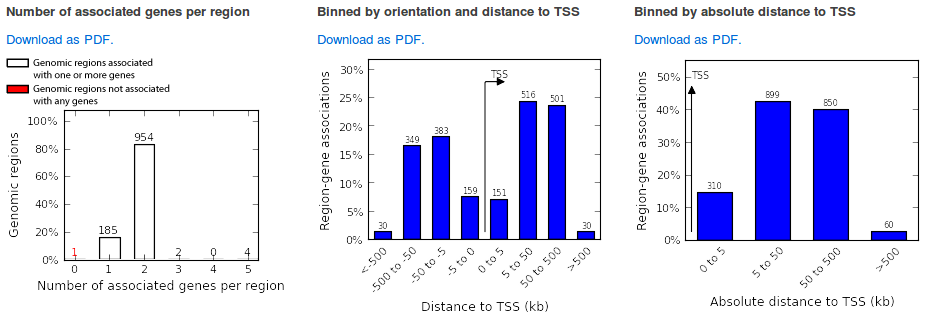
\includegraphics[width=\textwidth]{common}
\end{figure}


\begin{figure}[h]
	\caption{Motif for peaks of only GATA1}
	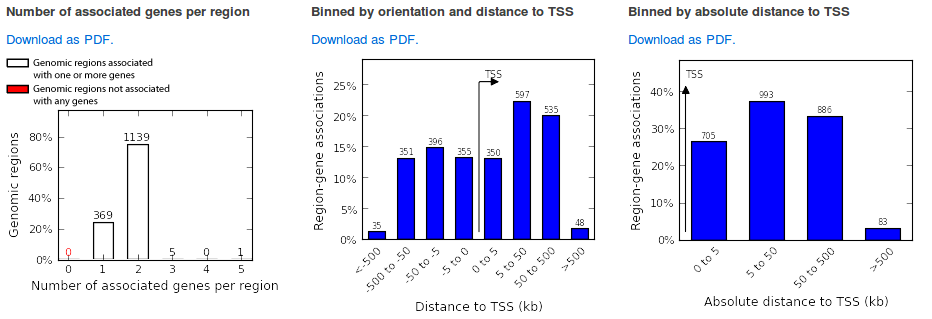
\includegraphics[width=\textwidth]{only_gata1}
\end{figure}
\end{document}

The tow figures have a comparable number of genes father than 5 kbases, however GATA1 has sensible more genes very close to the TSS.